\section{Data}
\subsection{JNI}
\begin{table}[H]
    \centering
    \label{tab:common:table:jni}
    \caption{Common table for JNI tests, Time(\textmu s)}
    \resizebox{\columnwidth}{!}{
        \rowcolors{1}{}{lightgray}
\begin{tabular}{lcccc}\toprule
\textbf{Block size}  & \textbf{No params} & \textbf{Vector} & \textbf{Convert} & \textbf{Columbia}\\\midrule
\textbf{16}  & 1.7922 $\pm$ 0.1392 & 1.9333 $\pm$ 0.1223 & 2.6052 $\pm$ 0.1004 & 4.1058 $\pm$ 0.3042\\
\textbf{32}  & 1.6983 $\pm$ 0.0220 & 2.8130 $\pm$ 1.7924 & 2.6006 $\pm$ 0.0370 & 3.9109 $\pm$ 0.0535\\
\textbf{64}  & 1.6755 $\pm$ 0.0149 & 1.6344 $\pm$ 0.1809 & 2.6630 $\pm$ 0.0425 & 3.9296 $\pm$ 0.0566\\
\textbf{128}  & 1.9604 $\pm$ 0.4978 & 1.2349 $\pm$ 0.1262 & 1.9375 $\pm$ 0.0843 & 3.0823 $\pm$ 0.0892\\
\textbf{256}  & 1.7292 $\pm$ 0.0694 & 1.3276 $\pm$ 0.2589 & 1.8141 $\pm$ 0.0276 & 3.0958 $\pm$ 0.0441\\
\textbf{512}  & 1.6916 $\pm$ 0.0110 & 1.2567 $\pm$ 0.1227 & 2.2818 $\pm$ 0.7011 & 3.1656 $\pm$ 0.0457\\
\textbf{1024}  & 2.0228 $\pm$ 0.5684 & 1.3167 $\pm$ 0.1341 & 6.3756 $\pm$ 8.4676 & 3.2896 $\pm$ 0.1396\\
\textbf{2048}  & 1.7218 $\pm$ 0.0288 & 1.5416 $\pm$ 0.1405 & 1.9099 $\pm$ 0.0898 & 3.4844 $\pm$ 0.1113\\
\textbf{4096}  & 1.1411 $\pm$ 0.0404 & 1.4010 $\pm$ 0.0788 & 2.0062 $\pm$ 0.1562 & 3.8562 $\pm$ 0.3197\\
\textbf{8192}  & 1.1105 $\pm$ 0.0078 & 1.4818 $\pm$ 0.0759 & 2.3671 $\pm$ 0.1897 & 3.8474 $\pm$ 0.4784\\
\textbf{16384}  & 1.1183 $\pm$ 0.0280 & 1.7308 $\pm$ 0.1043 & 2.5833 $\pm$ 0.1737 & 4.9724 $\pm$ 0.8955\\
\textbf{32768}  & 1.1162 $\pm$ 0.0084 & 2.2099 $\pm$ 0.1880 & 3.2062 $\pm$ 0.2029 & 5.3719 $\pm$ 0.2875\\
\textbf{65536}  & 1.7463 $\pm$ 1.2217 & 4.7474 $\pm$ 3.1960 & 4.3198 $\pm$ 0.2926 & 6.8136 $\pm$ 0.2499\\
\textbf{131072}  & 1.1027 $\pm$ 0.0141 & 2.6375 $\pm$ 0.1531 & 5.7004 $\pm$ 0.2681 & 9.6912 $\pm$ 1.4337\\
\textbf{262144} & 1.1006 $\pm$ 0.0118 & 3.3172 $\pm$ 0.1164 & 7.4630 $\pm$ 0.2309 & 10.2781 $\pm$ 0.2278\\
\bottomrule
\end{tabular}

    }
\end{table}

\subsection{Double Tables}

%%==================================================================
%% Double tables
%%==================================================================
\begin{table}[H]
    \centering
    \caption{Common table for \texttt{double} C++ FFT tests, Time(ms)}
    \label{tab:appendix:common:cpp}
    \resizebox{\columnwidth}{!}{
        \rowcolors{1}{}{lightgray}
\begin{tabular}{lrrrr}\toprule
\textbf{Block size}  & \textbf{Columbia Iterative} & \textbf{KISS} & \textbf{Princeton Iterative} & \textbf{Princeton Recursive}\\\midrule
\textbf{16}  & 0.0072 $\pm$ 0.0002 & 0.0056 $\pm$ 0.0002 & 0.0097 $\pm$ 0.0006 & 0.0202 $\pm$ 0.0008\\
\textbf{32}  & 0.0086 $\pm$ 0.0006 & 0.0069 $\pm$ 0.0002 & 0.0132 $\pm$ 0.0002 & 0.0368 $\pm$ 0.0008\\
\textbf{64}  & 0.0083 $\pm$ 0.0008 & 0.0079 $\pm$ 0.0002 & 0.0214 $\pm$ 0.0008 & 0.0705 $\pm$ 0.0022\\
\textbf{128}  & 0.0115 $\pm$ 0.0006 & 0.0131 $\pm$ 0.0006 & 0.0342 $\pm$ 0.0008 & 0.1434 $\pm$ 0.0012\\
\textbf{256}  & 0.0200 $\pm$ 0.0008 & 0.0182 $\pm$ 0.0008 & 0.0627 $\pm$ 0.0008 & 0.2978 $\pm$ 0.0025\\
\textbf{512}  & 0.0366 $\pm$ 0.0006 & 0.0461 $\pm$ 0.0022 & 0.1225 $\pm$ 0.0006 & 0.6379 $\pm$ 0.0035\\
\textbf{1024}  & 0.0773 $\pm$ 0.0020 & 0.0992 $\pm$ 0.0172 & 0.2744 $\pm$ 0.0098 & 1.3437 $\pm$ 0.0086\\
\textbf{2048}  & 0.2604 $\pm$ 0.0123 & 0.2047 $\pm$ 0.0149 & 0.5257 $\pm$ 0.0035 & 2.8773 $\pm$ 0.0253\\
\textbf{4096}  & 0.7974 $\pm$ 0.0216 & 0.4022 $\pm$ 0.0123 & 1.1701 $\pm$ 0.0118 & 6.1206 $\pm$ 0.0598\\
\textbf{8192}  & 1.9326 $\pm$ 0.0519 & 1.2470 $\pm$ 0.0451 & 2.5845 $\pm$ 0.0410 & 13.2345 $\pm$ 0.1433\\
\textbf{16384}  & 4.2789 $\pm$ 0.1254 & 2.3713 $\pm$ 0.0962 & 5.4518 $\pm$ 0.1149 & 27.6080 $\pm$ 0.1784\\
\textbf{32768}  & 9.9388 $\pm$ 0.3203 & 6.7420 $\pm$ 0.2534 & 12.2266 $\pm$ 0.4831 & 55.1227 $\pm$ 1.2277\\
\textbf{65536}  & 23.1031 $\pm$ 0.7648 & 16.0281 $\pm$ 0.3542 & 27.2805 $\pm$ 0.9530 & 102.1585 $\pm$ 3.5262\\
\textbf{131072}  & 75.4942 $\pm$ 1.6429 & 41.7620 $\pm$ 0.5968 & 78.9501 $\pm$ 1.9300 & 231.2663 $\pm$ 6.7357\\
\textbf{262144} & 243.8496 $\pm$ 1.0072 & 102.1196 $\pm$ 1.0817 & 250.4870 $\pm$ 5.2771 & 494.7038 $\pm$ 13.6690\\
\bottomrule
\end{tabular}

    }
\end{table}

\begin{table}[H]
    \centering
    \caption{Common table for \texttt{double} Java tests, Time(ms)}
    \label{tab:appendix:common:java}
    \rowcolors{1}{}{lightgray}
\begin{tabular}{lrrr}\toprule
\textbf{Block size}  & \textbf{Columbia Iterative} & \textbf{Princeton Iterative} & \textbf{Princeton Recursive}\\\midrule
\textbf{16}  & 0.03 $\pm$ 0.0010 & 0.12 $\pm$ 0.0053 & 0.13 $\pm$ 0.0108\\
\textbf{32}  & 0.08 $\pm$ 0.0033 & 0.13 $\pm$ 0.1198 & 0.06 $\pm$ 0.0035\\
\textbf{64}  & 0.02 $\pm$ 0.0125 & 0.09 $\pm$ 0.0468 & 0.13 $\pm$ 0.0043\\
\textbf{128}  & 0.01 $\pm$ 0.0002 & 0.14 $\pm$ 0.0020 & 0.49 $\pm$ 0.0486\\
\textbf{256}  & 0.02 $\pm$ 0.0008 & 0.56 $\pm$ 0.0947 & 0.69 $\pm$ 0.0325\\
\textbf{512}  & 0.06 $\pm$ 0.0010 & 0.87 $\pm$ 0.0615 & 1.75 $\pm$ 0.1245\\
\textbf{1024}  & 0.14 $\pm$ 0.0061 & 1.74 $\pm$ 0.0676 & 3.76 $\pm$ 0.2328\\
\textbf{2048}  & 0.43 $\pm$ 0.0159 & 4.40 $\pm$ 0.2064 & 8.69 $\pm$ 0.4575\\
\textbf{4096}  & 1.20 $\pm$ 0.0355 & 9.67 $\pm$ 0.4694 & 25.02 $\pm$ 0.8491\\
\textbf{8192}  & 2.87 $\pm$ 0.0637 & 22.96 $\pm$ 1.1025 & 52.08 $\pm$ 1.3973\\
\textbf{16384}  & 6.32 $\pm$ 0.2066 & 58.38 $\pm$ 1.9484 & 112.30 $\pm$ 1.6050\\
\textbf{32768}  & 12.26 $\pm$ 0.5700 & 150.72 $\pm$ 1.0864 & 239.07 $\pm$ 2.5276\\
\textbf{65536}  & 24.98 $\pm$ 0.9069 & 356.98 $\pm$ 1.5864 & 522.74 $\pm$ 6.1660\\
\textbf{131072}  & 85.94 $\pm$ 1.6097 & 815.86 $\pm$ 3.4304 & 1144.88 $\pm$ 17.8736\\
\textbf{262144} & 274.51 $\pm$ 5.1129 & 2108.07 $\pm$ 27.5366 & 2638.05 $\pm$ 40.5424\\
\bottomrule
\end{tabular}

\end{table}

\begin{table}[H]
    \centering
    \caption{Common table for \texttt{double} NEON tests, Time(ms)}
    \label{tab:appendix:common:neon}
    \rowcolors{1}{}{lightgray}
\begin{tabular}{lrr}\toprule
\textbf{Block size}  & \textbf{Iterative} & \textbf{Recursive}\\\midrule
\textbf{16}  & 0.005 $\pm$ 0.0004 & 0.010 $\pm$ 0.0006\\
\textbf{32}  & 0.005 $\pm$ 0.0002 & 0.015 $\pm$ 0.0010\\
\textbf{64}  & 0.005 $\pm$ 0.0002 & 0.018 $\pm$ 0.0014\\
\textbf{128}  & 0.008 $\pm$ 0.0002 & 0.028 $\pm$ 0.0016\\
\textbf{256}  & 0.013 $\pm$ 0.0008 & 0.054 $\pm$ 0.0076\\
\textbf{512}  & 0.034 $\pm$ 0.0006 & 0.096 $\pm$ 0.0014\\
\textbf{1024}  & 0.060 $\pm$ 0.0020 & 0.186 $\pm$ 0.0029\\
\textbf{2048}  & 0.192 $\pm$ 0.0176 & 0.365 $\pm$ 0.0082\\
\textbf{4096}  & 0.365 $\pm$ 0.0161 & 0.808 $\pm$ 0.0200\\
\textbf{8192}  & 1.005 $\pm$ 0.0129 & 1.613 $\pm$ 0.0278\\
\textbf{16384}  & 2.155 $\pm$ 0.0502 & 3.569 $\pm$ 0.0857\\
\textbf{32768}  & 4.789 $\pm$ 0.1543 & 7.600 $\pm$ 0.1878\\
\textbf{65536}  & 9.880 $\pm$ 0.2452 & 16.112 $\pm$ 0.3712\\
\textbf{131072}  & 27.815 $\pm$ 0.7146 & 34.165 $\pm$ 0.4722\\
\textbf{262144} & 63.185 $\pm$ 1.2662 & 74.074 $\pm$ 1.0666\\
\bottomrule
\end{tabular}

\end{table}

\subsection{Float Tables}
        
%%==================================================================
%% Float tables
%%==================================================================
\begin{table}[H]
    \centering
    \label{fig:appendix:java:common:float}
    \caption{Common table for \texttt{float} Java tests, Time(ms)}
    \rowcolors{1}{}{lightgray}
\begin{tabular}{lrrr}\toprule
\textbf{Block size}  & \textbf{Columbia Iterative} & \textbf{Princeton Iterative} & \textbf{Princeton Recursive}\\\midrule
\textbf{16}  & 0.0265 $\pm$ 0.0002 & 0.1398 $\pm$ 0.0906 & 0.0387 $\pm$ 0.0041\\
\textbf{32}  & 0.0658 $\pm$ 0.0029 & 0.0492 $\pm$ 0.0025 & 0.0850 $\pm$ 0.0078\\
\textbf{64}  & 0.0179 $\pm$ 0.0096 & 0.1078 $\pm$ 0.0067 & 0.1761 $\pm$ 0.0027\\
\textbf{128}  & 0.0158 $\pm$ 0.0022 & 0.1991 $\pm$ 0.0378 & 0.4199 $\pm$ 0.0237\\
\textbf{256}  & 0.0290 $\pm$ 0.0016 & 0.3547 $\pm$ 0.0104 & 0.8938 $\pm$ 0.0292\\
\textbf{512}  & 0.0603 $\pm$ 0.0014 & 0.7740 $\pm$ 0.1313 & 1.9155 $\pm$ 0.0437\\
\textbf{1024}  & 0.1289 $\pm$ 0.0027 & 1.7228 $\pm$ 0.1009 & 4.1350 $\pm$ 0.0866\\
\textbf{2048}  & 0.3302 $\pm$ 0.0182 & 3.8546 $\pm$ 0.2185 & 9.2740 $\pm$ 0.1674\\
\textbf{4096}  & 0.8200 $\pm$ 0.0272 & 8.8053 $\pm$ 0.4232 & 26.0912 $\pm$ 0.7752\\
\textbf{8192}  & 2.1766 $\pm$ 0.0639 & 21.1757 $\pm$ 0.6689 & 50.0776 $\pm$ 1.4876\\
\textbf{16384}  & 3.9995 $\pm$ 0.0902 & 46.8150 $\pm$ 1.0327 & 103.9682 $\pm$ 3.0954\\
\textbf{32768}  & 8.9846 $\pm$ 0.2566 & 113.1953 $\pm$ 3.9572 & 219.0208 $\pm$ 5.5642\\
\textbf{65536}  & 20.2833 $\pm$ 0.4786 & 261.9954 $\pm$ 9.1987 & 485.1020 $\pm$ 13.3737\\
\textbf{131072}  & 47.2950 $\pm$ 1.3073 & 622.4328 $\pm$ 24.9022 & 1039.4937 $\pm$ 26.9767\\
\textbf{262144} & 156.7135 $\pm$ 1.1934 & 1728.4640 $\pm$ 53.8042 & 2297.8011 $\pm$ 58.2951\\
\bottomrule
\end{tabular}

\end{table}

\begin{table}[H]
    \centering
    \label{fig:appendix:cpp:common:float}
    \caption{Common table for \texttt{float} C++ tests, Time(ms)}
    \rowcolors{1}{}{lightgray}
\begin{tabular}{lccc}\toprule
\textbf{Block size}  & \textbf{Columbia Iterative} & \textbf{Princeton Iterative} & \textbf{Princeton Recursive}\\\midrule
\textbf{16}  & 0.0049 $\pm$ 0.0004 & 0.0090 $\pm$ 0.0004 & 0.0215 $\pm$ 0.0043\\
\textbf{32}  & 0.0051 $\pm$ 0.0001 & 0.0128 $\pm$ 0.0010 & 0.0328 $\pm$ 0.0006\\
\textbf{64}  & 0.0052 $\pm$ 0.0002 & 0.0188 $\pm$ 0.0006 & 0.0617 $\pm$ 0.0010\\
\textbf{128}  & 0.0071 $\pm$ 0.0001 & 0.0292 $\pm$ 0.0006 & 0.1252 $\pm$ 0.0018\\
\textbf{256}  & 0.0160 $\pm$ 0.0080 & 0.0541 $\pm$ 0.0010 & 0.2642 $\pm$ 0.0078\\
\textbf{512}  & 0.0223 $\pm$ 0.0006 & 0.1038 $\pm$ 0.0012 & 0.5573 $\pm$ 0.0155\\
\textbf{1024}  & 0.0516 $\pm$ 0.0108 & 0.2082 $\pm$ 0.0025 & 1.1380 $\pm$ 0.0047\\
\textbf{2048}  & 0.1206 $\pm$ 0.0155 & 0.4536 $\pm$ 0.0106 & 2.4265 $\pm$ 0.0094\\
\textbf{4096}  & 0.8794 $\pm$ 0.0857 & 0.9690 $\pm$ 0.0061 & 5.1699 $\pm$ 0.0580\\
\textbf{8192}  & 1.8030 $\pm$ 0.1929 & 2.0605 $\pm$ 0.0110 & 10.7496 $\pm$ 0.0512\\
\textbf{16384}  & 2.9629 $\pm$ 0.1311 & 4.5027 $\pm$ 0.0341 & 22.8640 $\pm$ 0.1748\\
\textbf{32768}  & 8.2847 $\pm$ 0.2364 & 9.6797 $\pm$ 0.1288 & 48.0022 $\pm$ 0.2458\\
\textbf{65536}  & 18.8158 $\pm$ 0.5494 & 20.3049 $\pm$ 0.3467 & 96.9572 $\pm$ 0.2658\\
\textbf{131072}  & 43.7807 $\pm$ 1.2632 & 44.5770 $\pm$ 0.9577 & 192.4607 $\pm$ 5.9702\\
\textbf{262144} & 134.8093 $\pm$ 2.0115 & 129.5150 $\pm$ 1.8201 & 398.9698 $\pm$ 12.9207\\
\bottomrule
\end{tabular}

\end{table}

\begin{table}[H]
    \centering
    \caption{Common table for \texttt{float} NEON tests, Time(ms)}
    \label{tab:appendix:cpp:common:neon}
    \rowcolors{1}{}{lightgray}
\begin{tabular}{lrr}\toprule
\textbf{Block size}  & \textbf{Iterative} & \textbf{Recursive}\\\midrule
\textbf{16}  & 0.005 $\pm$ 0.0004 & 0.010 $\pm$ 0.0006\\
\textbf{32}  & 0.005 $\pm$ 0.0002 & 0.015 $\pm$ 0.0010\\
\textbf{64}  & 0.005 $\pm$ 0.0002 & 0.018 $\pm$ 0.0014\\
\textbf{128}  & 0.008 $\pm$ 0.0002 & 0.028 $\pm$ 0.0016\\
\textbf{256}  & 0.013 $\pm$ 0.0008 & 0.054 $\pm$ 0.0076\\
\textbf{512}  & 0.034 $\pm$ 0.0006 & 0.096 $\pm$ 0.0014\\
\textbf{1024}  & 0.060 $\pm$ 0.0020 & 0.186 $\pm$ 0.0029\\
\textbf{2048}  & 0.192 $\pm$ 0.0176 & 0.365 $\pm$ 0.0082\\
\textbf{4096}  & 0.365 $\pm$ 0.0161 & 0.808 $\pm$ 0.0200\\
\textbf{8192}  & 1.005 $\pm$ 0.0129 & 1.613 $\pm$ 0.0278\\
\textbf{16384}  & 2.155 $\pm$ 0.0502 & 3.569 $\pm$ 0.0857\\
\textbf{32768}  & 4.789 $\pm$ 0.1543 & 7.600 $\pm$ 0.1878\\
\textbf{65536}  & 9.880 $\pm$ 0.2452 & 16.112 $\pm$ 0.3712\\
\textbf{131072}  & 27.815 $\pm$ 0.7146 & 34.165 $\pm$ 0.4722\\
\textbf{262144} & 63.185 $\pm$ 1.2662 & 74.074 $\pm$ 1.0666\\
\bottomrule
\end{tabular}

\end{table}

\subsection{C++ Float graphs}

%%==================================================================
%% C++ Float graphs
%%==================================================================

\begin{table}[H]
    \centering
    \begin{tabular}{cc}
        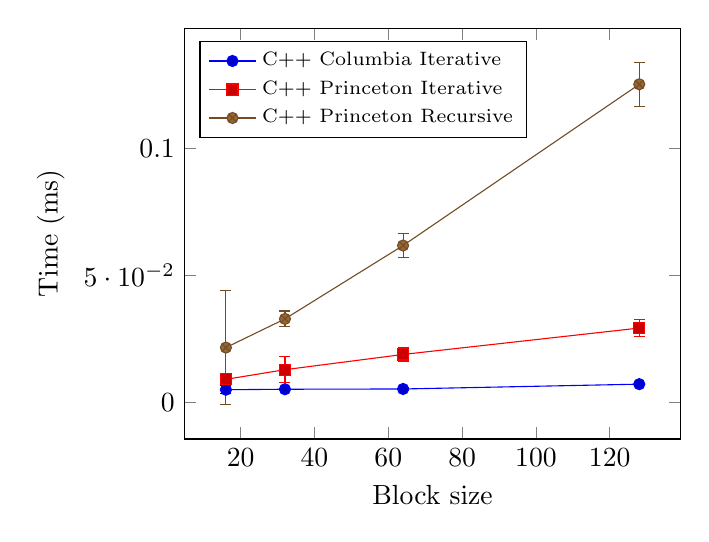
\begin{tikzpicture}
\begin{axis}[xlabel={Block size},ylabel={Time (ms)},width=0.65\linewidth,legend pos=north west,scaled y ticks = false,legend cell align=left,legend style={font=\scriptsize}]
\addplot+[error bars/.cd, y dir=both,y explicit] coordinates {
(16, 0.0049) +- (0.0015, 0.0015)
(32, 0.0051) +- (0.0002, 0.0002)
(64, 0.0052) +- (0.0005, 0.0005)
(128, 0.0071) +- (0.0003, 0.0003)
};
\addplot+[error bars/.cd, y dir=both,y explicit] coordinates {
(16, 0.0090) +- (0.0022, 0.0022)
(32, 0.0128) +- (0.0052, 0.0052)
(64, 0.0188) +- (0.0029, 0.0029)
(128, 0.0292) +- (0.0032, 0.0032)
};
\addplot+[error bars/.cd, y dir=both,y explicit] coordinates {
(16, 0.0215) +- (0.0225, 0.0225)
(32, 0.0328) +- (0.0031, 0.0031)
(64, 0.0617) +- (0.0047, 0.0047)
(128, 0.1252) +- (0.0086, 0.0086)
};
\legend{C++ Columbia Iterative , C++ Princeton Iterative , C++ Princeton Recursive}
\end{axis}
\end{tikzpicture}

        &
        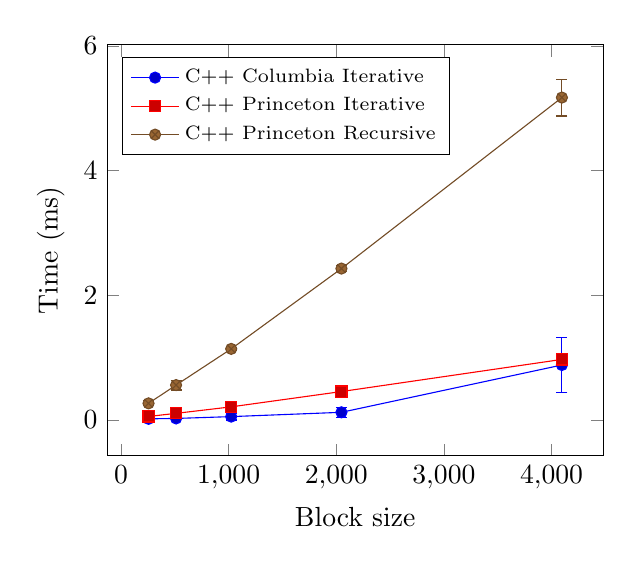
\begin{tikzpicture}
\begin{axis}[xlabel={Block size},ylabel={Time (ms)},width=0.65\linewidth,legend pos=north west,scaled y ticks = false,legend cell align=left,legend style={font=\scriptsize}]
\addplot+[error bars/.cd, y dir=both,y explicit] coordinates {
(256, 0.0160) +- (0.0408, 0.0408)
(512, 0.0223) +- (0.0032, 0.0032)
(1024, 0.0516) +- (0.0547, 0.0547)
(2048, 0.1206) +- (0.0787, 0.0787)
(4096, 0.8794) +- (0.4366, 0.4366)
};
\addplot+[error bars/.cd, y dir=both,y explicit] coordinates {
(256, 0.0541) +- (0.0048, 0.0048)
(512, 0.1038) +- (0.0056, 0.0056)
(1024, 0.2082) +- (0.0127, 0.0127)
(2048, 0.4536) +- (0.0536, 0.0536)
(4096, 0.9690) +- (0.0314, 0.0314)
};
\addplot+[error bars/.cd, y dir=both,y explicit] coordinates {
(256, 0.2642) +- (0.0405, 0.0405)
(512, 0.5573) +- (0.0791, 0.0791)
(1024, 1.1380) +- (0.0245, 0.0245)
(2048, 2.4265) +- (0.0476, 0.0476)
(4096, 5.1699) +- (0.2963, 0.2963)
};
\legend{C++ Columbia Iterative , C++ Princeton Iterative , C++ Princeton Recursive}
\end{axis}
\end{tikzpicture}

        \\
        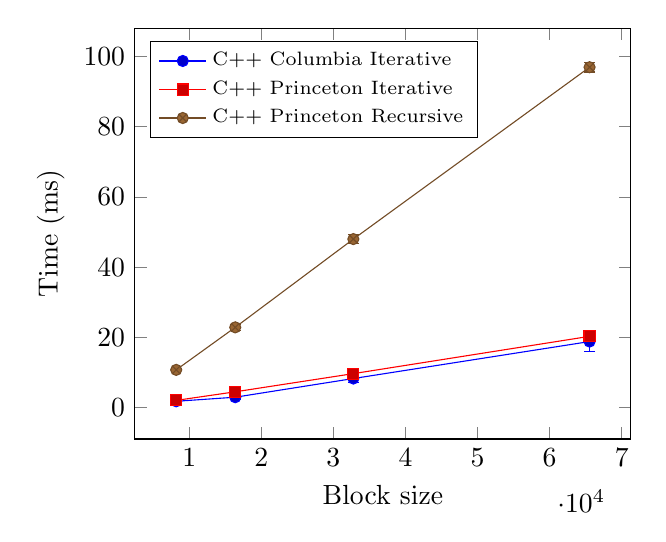
\begin{tikzpicture}
\begin{axis}[xlabel={Block size},ylabel={Time (ms)},width=0.65\linewidth,legend pos=north west,scaled y ticks = false,legend cell align=left,legend style={font=\scriptsize}]
\addplot+[error bars/.cd, y dir=both,y explicit] coordinates {
(8192, 1.8030) +- (0.9841, 0.9841)
(16384, 2.9629) +- (0.6687, 0.6687)
(32768, 8.2847) +- (1.2061, 1.2061)
(65536, 18.8158) +- (2.8032, 2.8032)
};
\addplot+[error bars/.cd, y dir=both,y explicit] coordinates {
(8192, 2.0605) +- (0.0561, 0.0561)
(16384, 4.5027) +- (0.1737, 0.1737)
(32768, 9.6797) +- (0.6568, 0.6568)
(65536, 20.3049) +- (1.7691, 1.7691)
};
\addplot+[error bars/.cd, y dir=both,y explicit] coordinates {
(8192, 10.7496) +- (0.2605, 0.2605)
(16384, 22.8640) +- (0.8917, 0.8917)
(32768, 48.0022) +- (1.2536, 1.2536)
(65536, 96.9572) +- (1.3564, 1.3564)
};
\legend{C++ Columbia Iterative , C++ Princeton Iterative , C++ Princeton Recursive}
\end{axis}
\end{tikzpicture}

        &
        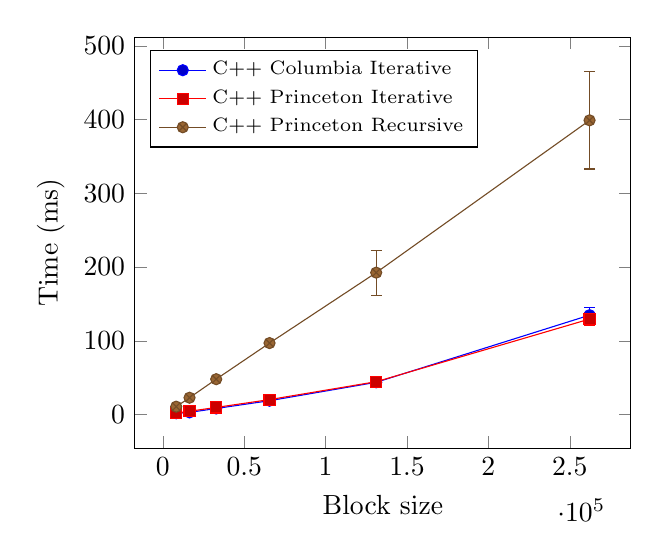
\begin{tikzpicture}
\begin{axis}[xlabel={Block size},ylabel={Time (ms)},width=0.65\linewidth,legend pos=north west,scaled y ticks = false,legend cell align=left,legend style={font=\scriptsize}]
\addplot+[error bars/.cd, y dir=both,y explicit] coordinates {
(8192, 1.8030) +- (0.9841, 0.9841)
(16384, 2.9629) +- (0.6687, 0.6687)
(32768, 8.2847) +- (1.2061, 1.2061)
(65536, 18.8158) +- (2.8032, 2.8032)
(131072, 43.7807) +- (6.4454, 6.4454)
(262144, 134.8093) +- (10.2633, 10.2633)
};
\addplot+[error bars/.cd, y dir=both,y explicit] coordinates {
(8192, 2.0605) +- (0.0561, 0.0561)
(16384, 4.5027) +- (0.1737, 0.1737)
(32768, 9.6797) +- (0.6568, 0.6568)
(65536, 20.3049) +- (1.7691, 1.7691)
(131072, 44.5770) +- (4.8859, 4.8859)
(262144, 129.5150) +- (9.2859, 9.2859)
};
\addplot+[error bars/.cd, y dir=both,y explicit] coordinates {
(8192, 10.7496) +- (0.2605, 0.2605)
(16384, 22.8640) +- (0.8917, 0.8917)
(32768, 48.0022) +- (1.2536, 1.2536)
(65536, 96.9572) +- (1.3564, 1.3564)
(131072, 192.4607) +- (30.4597, 30.4597)
(262144, 398.9698) +- (65.9217, 65.9217)
};
\legend{C++ Columbia Iterative , C++ Princeton Iterative , C++ Princeton Recursive}
\end{axis}
\end{tikzpicture}

    \end{tabular}
    \caption{\texttt{float} C++}
    \label{fig:appendix:float:cpp:line}
\end{table}

% \begin{figure}[H]
%     \centering
%     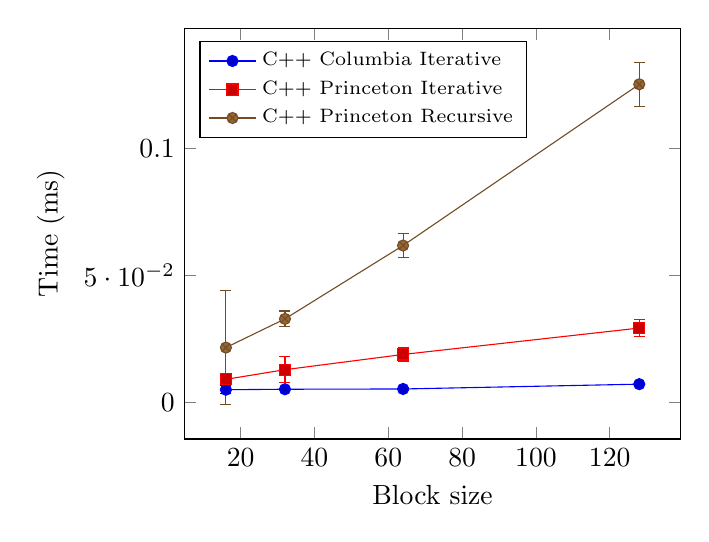
\begin{tikzpicture}
\begin{axis}[xlabel={Block size},ylabel={Time (ms)},width=0.65\linewidth,legend pos=north west,scaled y ticks = false,legend cell align=left,legend style={font=\scriptsize}]
\addplot+[error bars/.cd, y dir=both,y explicit] coordinates {
(16, 0.0049) +- (0.0015, 0.0015)
(32, 0.0051) +- (0.0002, 0.0002)
(64, 0.0052) +- (0.0005, 0.0005)
(128, 0.0071) +- (0.0003, 0.0003)
};
\addplot+[error bars/.cd, y dir=both,y explicit] coordinates {
(16, 0.0090) +- (0.0022, 0.0022)
(32, 0.0128) +- (0.0052, 0.0052)
(64, 0.0188) +- (0.0029, 0.0029)
(128, 0.0292) +- (0.0032, 0.0032)
};
\addplot+[error bars/.cd, y dir=both,y explicit] coordinates {
(16, 0.0215) +- (0.0225, 0.0225)
(32, 0.0328) +- (0.0031, 0.0031)
(64, 0.0617) +- (0.0047, 0.0047)
(128, 0.1252) +- (0.0086, 0.0086)
};
\legend{C++ Columbia Iterative , C++ Princeton Iterative , C++ Princeton Recursive}
\end{axis}
\end{tikzpicture}

%     \caption{\texttt{float} C++ small}
%     \label{fig:float:cpp:line:small}
% \end{figure}
% \begin{figure}[H]
%     \centering
%     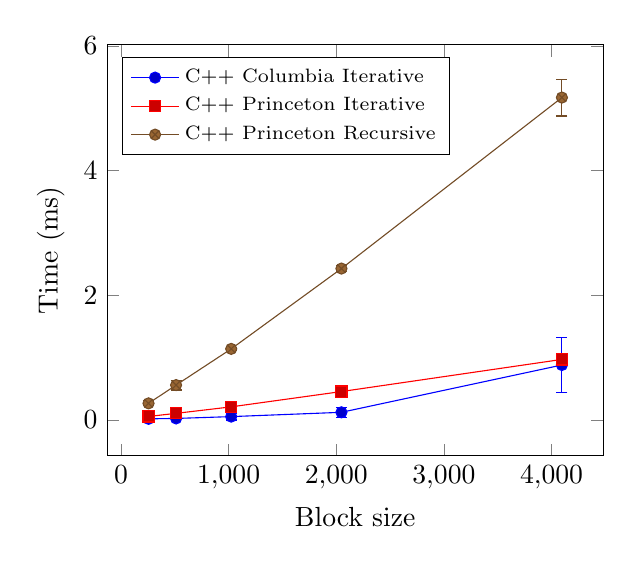
\begin{tikzpicture}
\begin{axis}[xlabel={Block size},ylabel={Time (ms)},width=0.65\linewidth,legend pos=north west,scaled y ticks = false,legend cell align=left,legend style={font=\scriptsize}]
\addplot+[error bars/.cd, y dir=both,y explicit] coordinates {
(256, 0.0160) +- (0.0408, 0.0408)
(512, 0.0223) +- (0.0032, 0.0032)
(1024, 0.0516) +- (0.0547, 0.0547)
(2048, 0.1206) +- (0.0787, 0.0787)
(4096, 0.8794) +- (0.4366, 0.4366)
};
\addplot+[error bars/.cd, y dir=both,y explicit] coordinates {
(256, 0.0541) +- (0.0048, 0.0048)
(512, 0.1038) +- (0.0056, 0.0056)
(1024, 0.2082) +- (0.0127, 0.0127)
(2048, 0.4536) +- (0.0536, 0.0536)
(4096, 0.9690) +- (0.0314, 0.0314)
};
\addplot+[error bars/.cd, y dir=both,y explicit] coordinates {
(256, 0.2642) +- (0.0405, 0.0405)
(512, 0.5573) +- (0.0791, 0.0791)
(1024, 1.1380) +- (0.0245, 0.0245)
(2048, 2.4265) +- (0.0476, 0.0476)
(4096, 5.1699) +- (0.2963, 0.2963)
};
\legend{C++ Columbia Iterative , C++ Princeton Iterative , C++ Princeton Recursive}
\end{axis}
\end{tikzpicture}

%     \caption{\texttt{float} C++ medium}
%     \label{fig:float:cpp:line:medium}
% \end{figure}
% \begin{figure}[H]
%     \centering
%     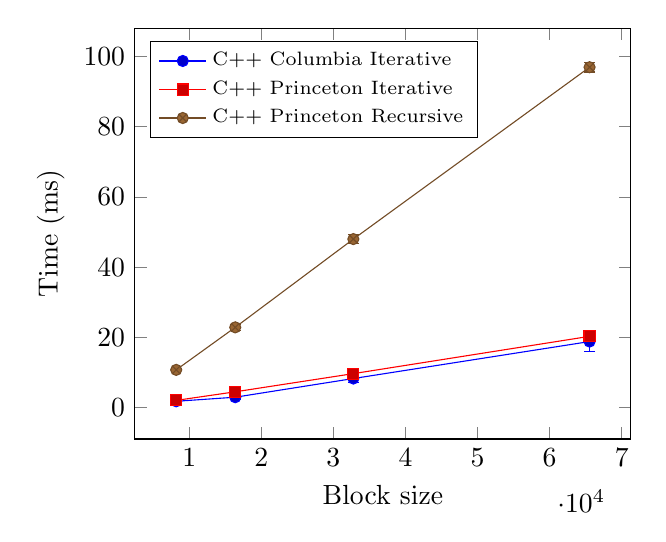
\begin{tikzpicture}
\begin{axis}[xlabel={Block size},ylabel={Time (ms)},width=0.65\linewidth,legend pos=north west,scaled y ticks = false,legend cell align=left,legend style={font=\scriptsize}]
\addplot+[error bars/.cd, y dir=both,y explicit] coordinates {
(8192, 1.8030) +- (0.9841, 0.9841)
(16384, 2.9629) +- (0.6687, 0.6687)
(32768, 8.2847) +- (1.2061, 1.2061)
(65536, 18.8158) +- (2.8032, 2.8032)
};
\addplot+[error bars/.cd, y dir=both,y explicit] coordinates {
(8192, 2.0605) +- (0.0561, 0.0561)
(16384, 4.5027) +- (0.1737, 0.1737)
(32768, 9.6797) +- (0.6568, 0.6568)
(65536, 20.3049) +- (1.7691, 1.7691)
};
\addplot+[error bars/.cd, y dir=both,y explicit] coordinates {
(8192, 10.7496) +- (0.2605, 0.2605)
(16384, 22.8640) +- (0.8917, 0.8917)
(32768, 48.0022) +- (1.2536, 1.2536)
(65536, 96.9572) +- (1.3564, 1.3564)
};
\legend{C++ Columbia Iterative , C++ Princeton Iterative , C++ Princeton Recursive}
\end{axis}
\end{tikzpicture}

%     \caption{\texttt{float} C++ large}
%     \label{fig:float:cpp:line:large}
% \end{figure}
% \begin{figure}[H]
%     \centering
%     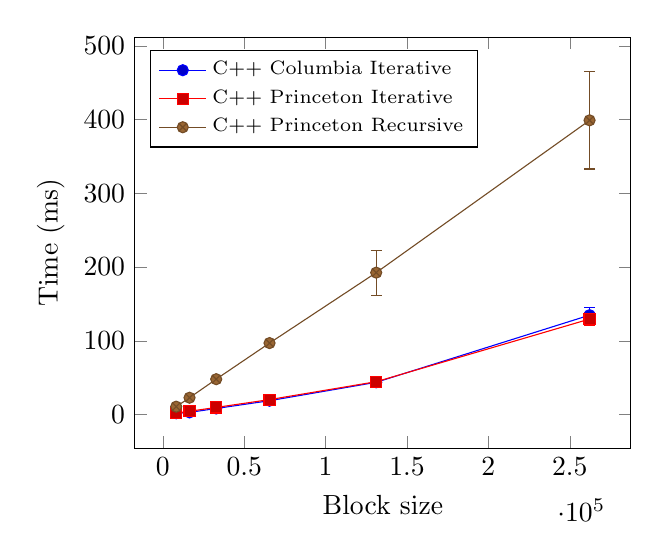
\begin{tikzpicture}
\begin{axis}[xlabel={Block size},ylabel={Time (ms)},width=0.65\linewidth,legend pos=north west,scaled y ticks = false,legend cell align=left,legend style={font=\scriptsize}]
\addplot+[error bars/.cd, y dir=both,y explicit] coordinates {
(8192, 1.8030) +- (0.9841, 0.9841)
(16384, 2.9629) +- (0.6687, 0.6687)
(32768, 8.2847) +- (1.2061, 1.2061)
(65536, 18.8158) +- (2.8032, 2.8032)
(131072, 43.7807) +- (6.4454, 6.4454)
(262144, 134.8093) +- (10.2633, 10.2633)
};
\addplot+[error bars/.cd, y dir=both,y explicit] coordinates {
(8192, 2.0605) +- (0.0561, 0.0561)
(16384, 4.5027) +- (0.1737, 0.1737)
(32768, 9.6797) +- (0.6568, 0.6568)
(65536, 20.3049) +- (1.7691, 1.7691)
(131072, 44.5770) +- (4.8859, 4.8859)
(262144, 129.5150) +- (9.2859, 9.2859)
};
\addplot+[error bars/.cd, y dir=both,y explicit] coordinates {
(8192, 10.7496) +- (0.2605, 0.2605)
(16384, 22.8640) +- (0.8917, 0.8917)
(32768, 48.0022) +- (1.2536, 1.2536)
(65536, 96.9572) +- (1.3564, 1.3564)
(131072, 192.4607) +- (30.4597, 30.4597)
(262144, 398.9698) +- (65.9217, 65.9217)
};
\legend{C++ Columbia Iterative , C++ Princeton Iterative , C++ Princeton Recursive}
\end{axis}
\end{tikzpicture}

%     \caption{\texttt{float} C++ extra}
%     \label{fig:float:cpp:line:extra}
% \end{figure}

\subsection{Java Float graphs}
%%==================================================================
%% Java Float graphs
%%==================================================================
\begin{table}[H]
    \centering
    \begin{tabular}{cc}
        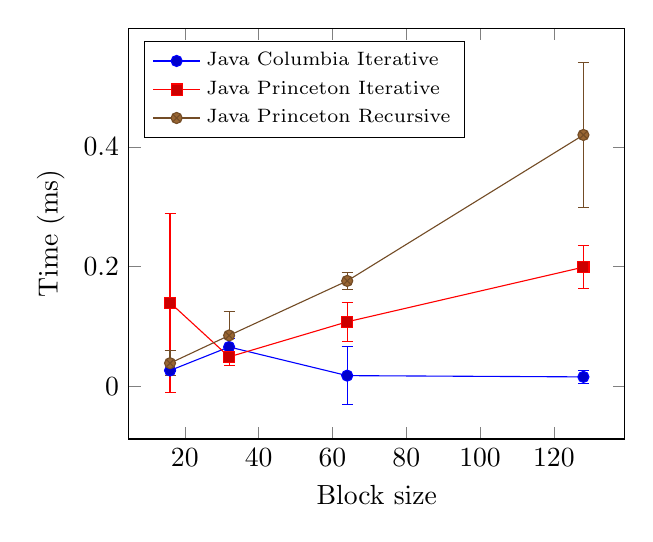
\begin{tikzpicture}
\begin{axis}[xlabel={Block size},ylabel={Time (ms)},width=0.65\linewidth,legend pos=north west,scaled y ticks = false,legend cell align=left,legend style={font=\scriptsize}]
\addplot+[error bars/.cd, y dir=both,y explicit] coordinates {
(16, 0.0265) +- (0.0011, 0.0011)
(32, 0.0658) +- (0.0148, 0.0148)
(64, 0.0179) +- (0.0486, 0.0486)
(128, 0.0158) +- (0.0105, 0.0105)
};
\addplot+[error bars/.cd, y dir=both,y explicit] coordinates {
(16, 0.1398) +- (0.1496, 0.1496)
(32, 0.0492) +- (0.0139, 0.0139)
(64, 0.1078) +- (0.0326, 0.0326)
(128, 0.1991) +- (0.0359, 0.0359)
};
\addplot+[error bars/.cd, y dir=both,y explicit] coordinates {
(16, 0.0387) +- (0.0210, 0.0210)
(32, 0.0850) +- (0.0396, 0.0396)
(64, 0.1761) +- (0.0136, 0.0136)
(128, 0.4199) +- (0.1211, 0.1211)
};
\legend{Java Columbia Iterative , Java Princeton Iterative , Java Princeton Recursive}
\end{axis}
\end{tikzpicture}

        &
        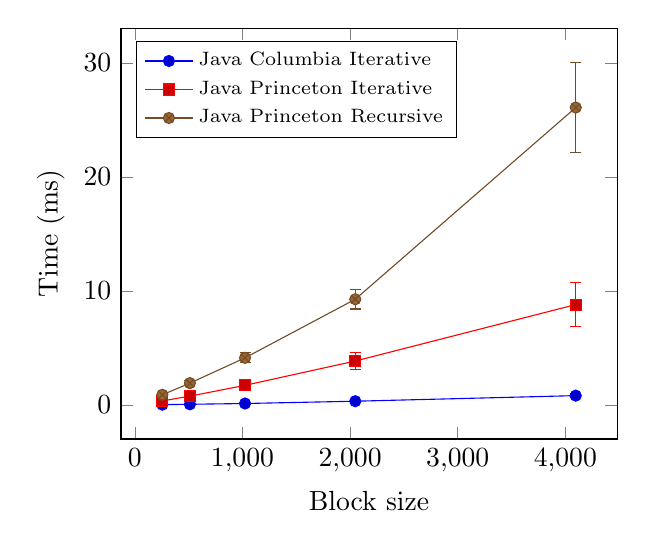
\begin{tikzpicture}
\begin{axis}[xlabel={Block size},ylabel={Time (ms)},width=0.65\linewidth,legend pos=north west,scaled y ticks = false,legend cell align=left,legend style={font=\scriptsize}]
\addplot+[error bars/.cd, y dir=both,y explicit] coordinates {
(256, 0.0290) +- (0.0075, 0.0075)
(512, 0.0603) +- (0.0073, 0.0073)
(1024, 0.1289) +- (0.0141, 0.0141)
(2048, 0.3302) +- (0.0926, 0.0926)
(4096, 0.8200) +- (0.1385, 0.1385)
};
\addplot+[error bars/.cd, y dir=both,y explicit] coordinates {
(256, 0.3547) +- (0.1008, 0.1008)
(512, 0.7740) +- (0.1657, 0.1657)
(1024, 1.7228) +- (0.2675, 0.2675)
(2048, 3.8546) +- (0.7268, 0.7268)
(4096, 8.8053) +- (1.9485, 1.9485)
};
\addplot+[error bars/.cd, y dir=both,y explicit] coordinates {
(256, 0.8938) +- (0.1489, 0.1489)
(512, 1.9155) +- (0.2226, 0.2226)
(1024, 4.1350) +- (0.4424, 0.4424)
(2048, 9.2740) +- (0.8540, 0.8540)
(4096, 26.0912) +- (3.9554, 3.9554)
};
\legend{Java Columbia Iterative , Java Princeton Iterative , Java Princeton Recursive}
\end{axis}
\end{tikzpicture}

        \\
        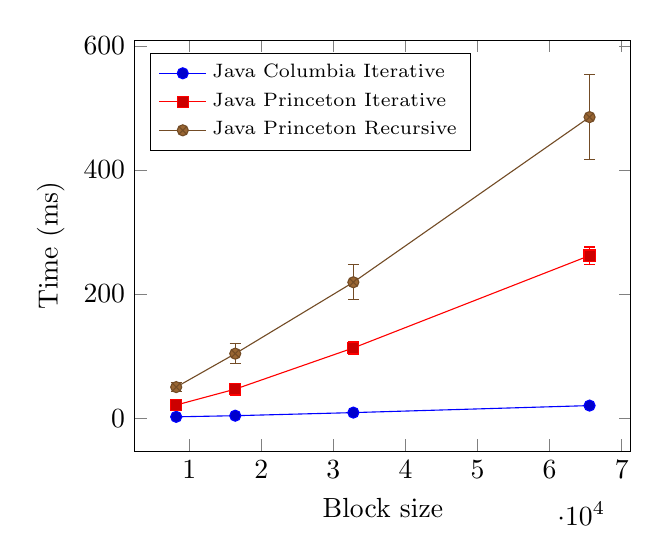
\begin{tikzpicture}
\begin{axis}[xlabel={Block size},ylabel={Time (ms)},width=0.65\linewidth,legend pos=north west,scaled y ticks = false,legend cell align=left,legend style={font=\scriptsize}]
\addplot+[error bars/.cd, y dir=both,y explicit] coordinates {
(8192, 2.1766) +- (0.3256, 0.3256)
(16384, 3.9995) +- (0.4596, 0.4596)
(32768, 8.9846) +- (1.3089, 1.3089)
(65536, 20.2833) +- (2.4423, 2.4423)
};
\addplot+[error bars/.cd, y dir=both,y explicit] coordinates {
(8192, 21.1757) +- (4.9079, 4.9079)
(16384, 46.8150) +- (9.6619, 9.6619)
(32768, 113.1953) +- (11.0218, 11.0218)
(65536, 261.9954) +- (13.8293, 13.8293)
};
\addplot+[error bars/.cd, y dir=both,y explicit] coordinates {
(8192, 50.0776) +- (7.5896, 7.5896)
(16384, 103.9682) +- (15.7929, 15.7929)
(32768, 219.0208) +- (28.3890, 28.3890)
(65536, 485.1020) +- (68.2330, 68.2330)
};
\legend{Java Columbia Iterative , Java Princeton Iterative , Java Princeton Recursive}
\end{axis}
\end{tikzpicture}

        &
        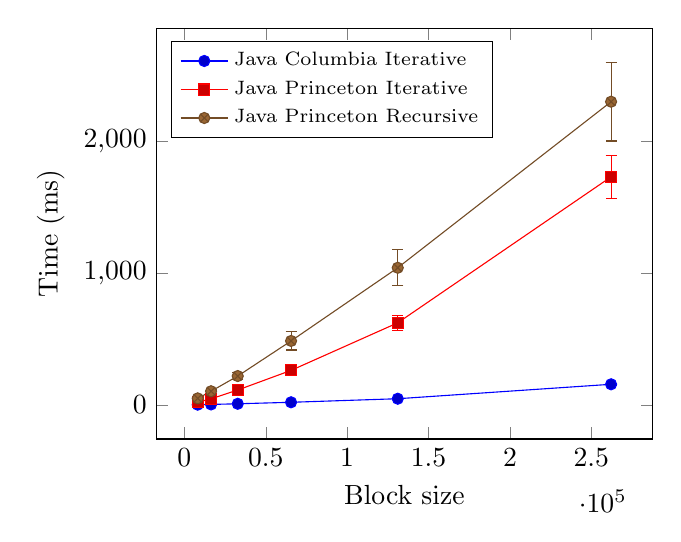
\begin{tikzpicture}
\begin{axis}[xlabel={Block size},ylabel={Time (ms)},width=0.65\linewidth,legend pos=north west,scaled y ticks = false,legend cell align=left,legend style={font=\scriptsize}]
\addplot+[error bars/.cd, y dir=both,y explicit] coordinates {
(8192, 2.1766) +- (0.3256, 0.3256)
(16384, 3.9995) +- (0.4596, 0.4596)
(32768, 8.9846) +- (1.3089, 1.3089)
(65536, 20.2833) +- (2.4423, 2.4423)
(131072, 47.2950) +- (6.6700, 6.6700)
(262144, 156.7135) +- (6.0892, 6.0892)
};
\addplot+[error bars/.cd, y dir=both,y explicit] coordinates {
(8192, 21.1757) +- (4.9079, 4.9079)
(16384, 46.8150) +- (9.6619, 9.6619)
(32768, 113.1953) +- (11.0218, 11.0218)
(65536, 261.9954) +- (13.8293, 13.8293)
(131072, 622.4328) +- (57.9001, 57.9001)
(262144, 1728.4640) +- (161.0712, 161.0712)
};
\addplot+[error bars/.cd, y dir=both,y explicit] coordinates {
(8192, 50.0776) +- (7.5896, 7.5896)
(16384, 103.9682) +- (15.7929, 15.7929)
(32768, 219.0208) +- (28.3890, 28.3890)
(65536, 485.1020) +- (68.2330, 68.2330)
(131072, 1039.4937) +- (137.6356, 137.6356)
(262144, 2297.8011) +- (297.4241, 297.4241)
};
\legend{Java Columbia Iterative , Java Princeton Iterative , Java Princeton Recursive}
\end{axis}
\end{tikzpicture}

    \end{tabular}
    \caption{\texttt{float} Java}
    \label{fig:appendix:float:java:line}
\end{table}

% \begin{figure}[H]
%     \centering
%     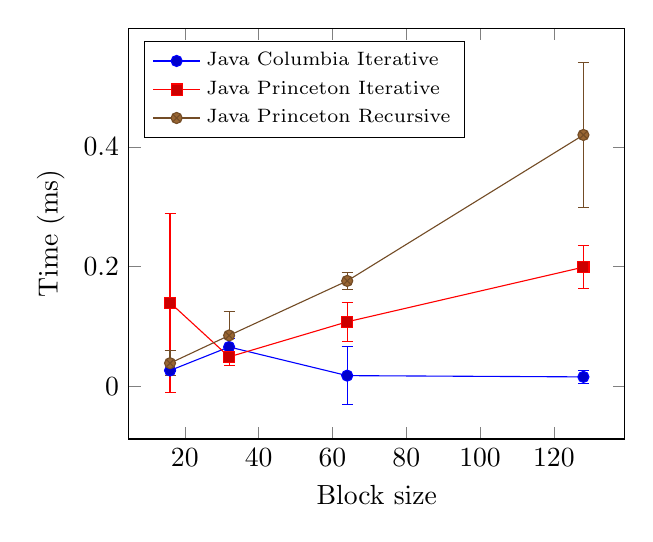
\begin{tikzpicture}
\begin{axis}[xlabel={Block size},ylabel={Time (ms)},width=0.65\linewidth,legend pos=north west,scaled y ticks = false,legend cell align=left,legend style={font=\scriptsize}]
\addplot+[error bars/.cd, y dir=both,y explicit] coordinates {
(16, 0.0265) +- (0.0011, 0.0011)
(32, 0.0658) +- (0.0148, 0.0148)
(64, 0.0179) +- (0.0486, 0.0486)
(128, 0.0158) +- (0.0105, 0.0105)
};
\addplot+[error bars/.cd, y dir=both,y explicit] coordinates {
(16, 0.1398) +- (0.1496, 0.1496)
(32, 0.0492) +- (0.0139, 0.0139)
(64, 0.1078) +- (0.0326, 0.0326)
(128, 0.1991) +- (0.0359, 0.0359)
};
\addplot+[error bars/.cd, y dir=both,y explicit] coordinates {
(16, 0.0387) +- (0.0210, 0.0210)
(32, 0.0850) +- (0.0396, 0.0396)
(64, 0.1761) +- (0.0136, 0.0136)
(128, 0.4199) +- (0.1211, 0.1211)
};
\legend{Java Columbia Iterative , Java Princeton Iterative , Java Princeton Recursive}
\end{axis}
\end{tikzpicture}

%     \caption{\texttt{float} Java small}
%     \label{fig:float:java:line:small}
% \end{figure}
% \begin{figure}[H]
%     \centering
%     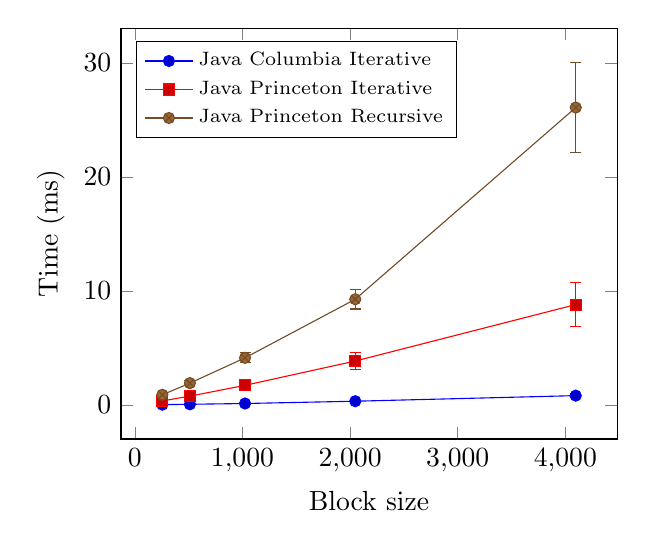
\begin{tikzpicture}
\begin{axis}[xlabel={Block size},ylabel={Time (ms)},width=0.65\linewidth,legend pos=north west,scaled y ticks = false,legend cell align=left,legend style={font=\scriptsize}]
\addplot+[error bars/.cd, y dir=both,y explicit] coordinates {
(256, 0.0290) +- (0.0075, 0.0075)
(512, 0.0603) +- (0.0073, 0.0073)
(1024, 0.1289) +- (0.0141, 0.0141)
(2048, 0.3302) +- (0.0926, 0.0926)
(4096, 0.8200) +- (0.1385, 0.1385)
};
\addplot+[error bars/.cd, y dir=both,y explicit] coordinates {
(256, 0.3547) +- (0.1008, 0.1008)
(512, 0.7740) +- (0.1657, 0.1657)
(1024, 1.7228) +- (0.2675, 0.2675)
(2048, 3.8546) +- (0.7268, 0.7268)
(4096, 8.8053) +- (1.9485, 1.9485)
};
\addplot+[error bars/.cd, y dir=both,y explicit] coordinates {
(256, 0.8938) +- (0.1489, 0.1489)
(512, 1.9155) +- (0.2226, 0.2226)
(1024, 4.1350) +- (0.4424, 0.4424)
(2048, 9.2740) +- (0.8540, 0.8540)
(4096, 26.0912) +- (3.9554, 3.9554)
};
\legend{Java Columbia Iterative , Java Princeton Iterative , Java Princeton Recursive}
\end{axis}
\end{tikzpicture}

%     \caption{\texttt{float} Java medium}
%     \label{fig:float:java:line:medium}
% \end{figure}
% \begin{figure}[H]
%     \centering
%     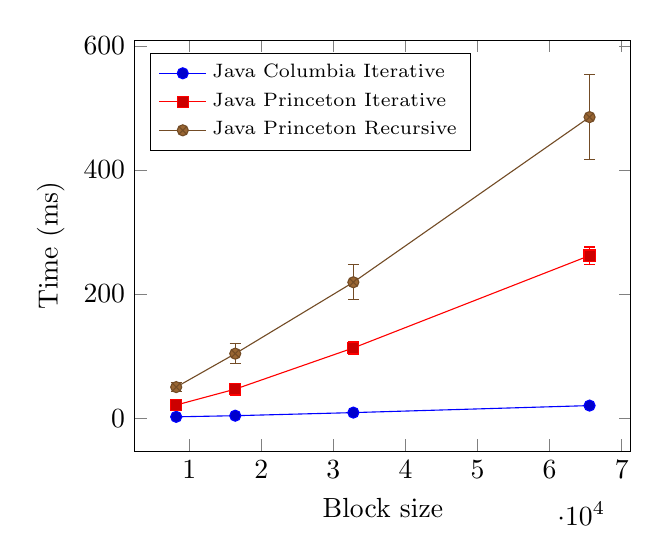
\begin{tikzpicture}
\begin{axis}[xlabel={Block size},ylabel={Time (ms)},width=0.65\linewidth,legend pos=north west,scaled y ticks = false,legend cell align=left,legend style={font=\scriptsize}]
\addplot+[error bars/.cd, y dir=both,y explicit] coordinates {
(8192, 2.1766) +- (0.3256, 0.3256)
(16384, 3.9995) +- (0.4596, 0.4596)
(32768, 8.9846) +- (1.3089, 1.3089)
(65536, 20.2833) +- (2.4423, 2.4423)
};
\addplot+[error bars/.cd, y dir=both,y explicit] coordinates {
(8192, 21.1757) +- (4.9079, 4.9079)
(16384, 46.8150) +- (9.6619, 9.6619)
(32768, 113.1953) +- (11.0218, 11.0218)
(65536, 261.9954) +- (13.8293, 13.8293)
};
\addplot+[error bars/.cd, y dir=both,y explicit] coordinates {
(8192, 50.0776) +- (7.5896, 7.5896)
(16384, 103.9682) +- (15.7929, 15.7929)
(32768, 219.0208) +- (28.3890, 28.3890)
(65536, 485.1020) +- (68.2330, 68.2330)
};
\legend{Java Columbia Iterative , Java Princeton Iterative , Java Princeton Recursive}
\end{axis}
\end{tikzpicture}

%     \caption{\texttt{float} Java large}
%     \label{fig:float:java:line:large}
% \end{figure}
% \begin{figure}[H]
%     \centering
%     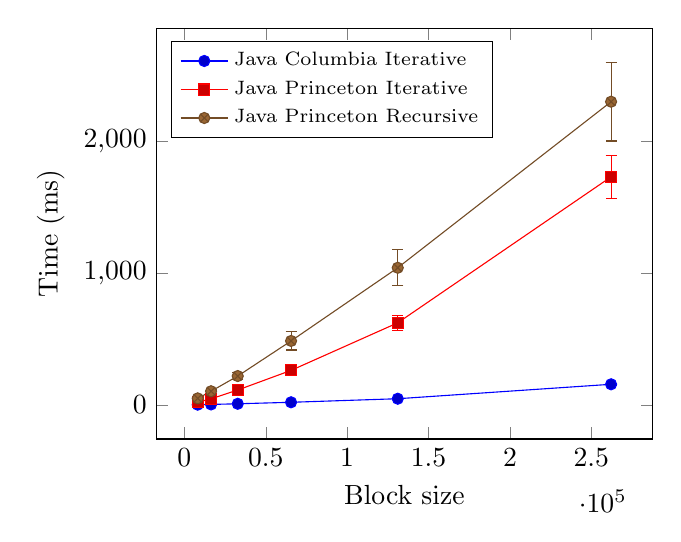
\begin{tikzpicture}
\begin{axis}[xlabel={Block size},ylabel={Time (ms)},width=0.65\linewidth,legend pos=north west,scaled y ticks = false,legend cell align=left,legend style={font=\scriptsize}]
\addplot+[error bars/.cd, y dir=both,y explicit] coordinates {
(8192, 2.1766) +- (0.3256, 0.3256)
(16384, 3.9995) +- (0.4596, 0.4596)
(32768, 8.9846) +- (1.3089, 1.3089)
(65536, 20.2833) +- (2.4423, 2.4423)
(131072, 47.2950) +- (6.6700, 6.6700)
(262144, 156.7135) +- (6.0892, 6.0892)
};
\addplot+[error bars/.cd, y dir=both,y explicit] coordinates {
(8192, 21.1757) +- (4.9079, 4.9079)
(16384, 46.8150) +- (9.6619, 9.6619)
(32768, 113.1953) +- (11.0218, 11.0218)
(65536, 261.9954) +- (13.8293, 13.8293)
(131072, 622.4328) +- (57.9001, 57.9001)
(262144, 1728.4640) +- (161.0712, 161.0712)
};
\addplot+[error bars/.cd, y dir=both,y explicit] coordinates {
(8192, 50.0776) +- (7.5896, 7.5896)
(16384, 103.9682) +- (15.7929, 15.7929)
(32768, 219.0208) +- (28.3890, 28.3890)
(65536, 485.1020) +- (68.2330, 68.2330)
(131072, 1039.4937) +- (137.6356, 137.6356)
(262144, 2297.8011) +- (297.4241, 297.4241)
};
\legend{Java Columbia Iterative , Java Princeton Iterative , Java Princeton Recursive}
\end{axis}
\end{tikzpicture}

%     \caption{\texttt{float} Java extra}
%     \label{fig:float:java:line:extra}
% \end{figure}




%
% \begin{table}[H]
%     \centering
%     \label{tab:common:table:cpp}
%     \caption{Common table for C++ tests, Time (ms)}
%     \resizebox{\columnwidth}{!}{
%         \begin{tabular}{|l|c|c|c|c|c|}\hline
\textbf{Block size}  & \textbf{Columbia converted Iterative} & \textbf{Columbia optimized Iterative} & \textbf{KISS} & \textbf{Princeton converted Iterative} & \textbf{Princeton converted Recursive}\\\hline
\textbf{16}  & 0.0225 $\pm$ 0.0033 & 0.0198 $\pm$ 0.0025 & 0.0195 $\pm$ 0.0067 & 0.0342 $\pm$ 0.0053 & 0.0612 $\pm$ 0.0065\\\hline
\textbf{32}  & 0.0322 $\pm$ 0.0025 & 0.0322 $\pm$ 0.0031 & 0.0239 $\pm$ 0.0031 & 0.0545 $\pm$ 0.0043 & 0.1085 $\pm$ 0.0020\\\hline
\textbf{64}  & 0.0525 $\pm$ 0.0014 & 0.0524 $\pm$ 0.0012 & 0.0338 $\pm$ 0.0020 & 0.0847 $\pm$ 0.0059 & 0.2148 $\pm$ 0.0024\\\hline
\textbf{128}  & 0.1025 $\pm$ 0.0033 & 0.0814 $\pm$ 0.0127 & 0.0629 $\pm$ 0.0084 & 0.1328 $\pm$ 0.0029 & 0.4517 $\pm$ 0.0057\\\hline
\textbf{256}  & 0.0925 $\pm$ 0.0178 & 0.0822 $\pm$ 0.0039 & 0.1158 $\pm$ 0.0035 & 0.2807 $\pm$ 0.0073 & 0.9139 $\pm$ 0.0067\\\hline
\textbf{512}  & 0.1709 $\pm$ 0.0267 & 0.1744 $\pm$ 0.0308 & 0.2109 $\pm$ 0.0049 & 0.5486 $\pm$ 0.0253 & 1.9142 $\pm$ 0.0102\\\hline
\textbf{1024}  & 0.3656 $\pm$ 0.0284 & 0.3397 $\pm$ 0.0108 & 0.4072 $\pm$ 0.0086 & 1.1691 $\pm$ 0.0172 & 4.0665 $\pm$ 0.0127\\\hline
\textbf{2048}  & 0.9177 $\pm$ 0.0541 & 0.7402 $\pm$ 0.0190 & 0.8635 $\pm$ 0.0243 & 2.4714 $\pm$ 0.0188 & 8.7235 $\pm$ 0.0725\\\hline
\textbf{4096}  & 1.6737 $\pm$ 0.0461 & 1.9889 $\pm$ 0.0982 & 1.9558 $\pm$ 0.1347 & 5.3867 $\pm$ 0.1000 & 18.3487 $\pm$ 0.1235\\\hline
\textbf{8192}  & 3.7768 $\pm$ 0.1838 & 3.8584 $\pm$ 0.2236 & 3.8499 $\pm$ 0.1603 & 11.7050 $\pm$ 0.5076 & 38.4780 $\pm$ 0.6441\\\hline
\textbf{16384}  & 8.2947 $\pm$ 0.3759 & 8.5556 $\pm$ 0.5672 & 7.8854 $\pm$ 0.2775 & 24.3807 $\pm$ 0.5902 & 80.4920 $\pm$ 0.8228\\\hline
\textbf{32768}  & 19.1886 $\pm$ 1.1809 & 18.5907 $\pm$ 0.9959 & 17.6197 $\pm$ 0.5490 & 52.3713 $\pm$ 1.1313 & 167.3867 $\pm$ 1.5300\\\hline
\textbf{65536} & 42.8520 $\pm$ 1.4120 & 44.2337 $\pm$ 2.4361 & 38.3601 $\pm$ 0.7332 & 112.4273 $\pm$ 1.1197 & 346.7600 $\pm$ 1.9190\\\hline
\end{tabular}

%     }
% \end{table}
%
% \begin{table}[H]
%     \centering
%     \label{tab:common:table:java}
%     \caption{Common table for Java tests, Time (ms)}
%     \resizebox{\columnwidth}{!}{
%         \begin{tabular}{|l|c|c|c|}\hline
\textbf{Block size}  & \textbf{Columbia Iterative} & \textbf{Princeton Iterative} & \textbf{Princeton Recursive}\\\hline
\textbf{16}  & 0.0210 $\pm$ 0.0008 & 0.1738 $\pm$ 0.0368 & 0.2730 $\pm$ 0.0708\\\hline
\textbf{32}  & 0.0429 $\pm$ 0.0018 & 0.0571 $\pm$ 0.0071 & 0.3983 $\pm$ 0.0568\\\hline
\textbf{64}  & 0.0906 $\pm$ 0.0010 & 0.0916 $\pm$ 0.0073 & 0.2104 $\pm$ 0.0402\\\hline
\textbf{128}  & 0.2233 $\pm$ 0.0382 & 0.2353 $\pm$ 0.0339 & 0.3204 $\pm$ 0.0425\\\hline
\textbf{256}  & 0.0372 $\pm$ 0.0022 & 0.4380 $\pm$ 0.0316 & 0.7415 $\pm$ 0.0431\\\hline
\textbf{512}  & 0.0754 $\pm$ 0.0029 & 0.9865 $\pm$ 0.0672 & 1.7743 $\pm$ 0.1944\\\hline
\textbf{1024}  & 0.1507 $\pm$ 0.0059 & 2.0255 $\pm$ 0.0933 & 3.5339 $\pm$ 0.2466\\\hline
\textbf{2048}  & 0.4299 $\pm$ 0.0312 & 4.5366 $\pm$ 0.3038 & 8.2740 $\pm$ 0.6905\\\hline
\textbf{4096}  & 0.9984 $\pm$ 0.0915 & 10.6191 $\pm$ 0.8679 & 17.9445 $\pm$ 0.9022\\\hline
\textbf{8192}  & 2.3125 $\pm$ 0.2709 & 27.5617 $\pm$ 1.9755 & 37.6118 $\pm$ 1.5008\\\hline
\textbf{16384}  & 4.8597 $\pm$ 0.4114 & 62.6869 $\pm$ 1.7191 & 80.1848 $\pm$ 1.9414\\\hline
\textbf{32768}  & 11.2535 $\pm$ 0.9718 & 155.5247 $\pm$ 2.7411 & 172.5062 $\pm$ 2.2489\\\hline
\textbf{65536} & 26.3906 $\pm$ 2.1662 & 366.0557 $\pm$ 2.8910 & 366.6833 $\pm$ 3.3610\\\hline
\end{tabular}

%     }
% \end{table}
%
% \begin{table}[H]
%     \centering
%     \label{tab:jni:convert}
%     \caption{JNI convert, Time (textmu s)}
%     \input{Data/results/JNI/Benchmark_convert.tex}
% \end{table}
%
% \begin{table}[H]
%     \centering
%     \label{tab:jni:no:params}
%     \caption{JNI no parameters, Time (textmu s)}
%     \input{Data/results/JNI/Benchmark_no_params.tex}
% \end{table}
%
% \begin{table}[H]
%     \centering
%     \label{tab:jni:vector}
%     \caption{JNI convert, Time (textmu s)}
%     \input{Data/results/JNI/Benchmark_vector.tex}
% \end{table}
%
% \begin{table}[H]
%     \centering
%     \label{tab:java:princeton:iterative}
%     \caption{Java Princeton Iterative, Time (ms)}
%     /home/algo/Skola/Exjobb/Data/results/FFT/Java_Princeton_Iterative_N_30.tex
% \end{table}
%
% \begin{table}[H]
%     \centering
%     \label{tab:java:princeton:recursive}
%     \caption{Java Princeton Recursive, Time (ms)}
%     \input{Data/results/FFT/Java_Princeton_Recursive.tex}
% \end{table}
%
% \begin{table}[H]
%     \centering
%     \label{tab:java:columbia:iterative}
%     \caption{Java Columbia Iterative, Time (ms)}
%     /home/algo/Skola/Exjobb/Data/results/FFT/Java_Columbia_Iterative_N_30.tex
% \end{table}
%
% \begin{table}[H]
%     \centering
%     \label{tab:cpp:princeton:iterative}
%     \caption{C++ Princeton Iterative, Time (ms)}
%     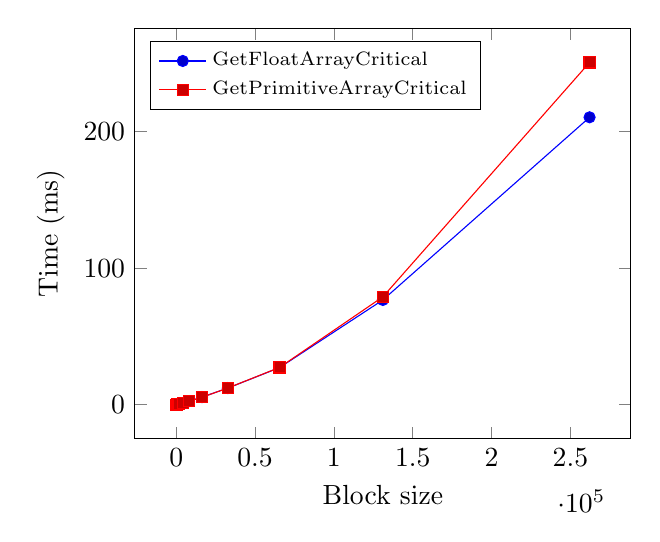
\begin{tikzpicture}
\begin{axis}[xlabel={Block size},ylabel={Time (ms)},width=0.65\linewidth,legend pos=north west,scaled y ticks = false,legend cell align=left,legend style={font=\scriptsize}]
\addplot coordinates {
(16, 0.0083)
(32, 0.0124)
(64, 0.0201)
(128, 0.0348)
(256, 0.0651)
(512, 0.1275)
(1024, 0.2659)
(2048, 0.5235)
(4096, 1.1475)
(8192, 2.6441)
(16384, 5.5785)
(32768, 12.1775)
(65536, 27.1549)
(131072, 76.6735)
(262144, 210.3414)
};
\addplot coordinates {
(16, 0.0097)
(32, 0.0132)
(64, 0.0214)
(128, 0.0342)
(256, 0.0627)
(512, 0.1225)
(1024, 0.2744)
(2048, 0.5257)
(4096, 1.1701)
(8192, 2.5845)
(16384, 5.4518)
(32768, 12.2266)
(65536, 27.2805)
(131072, 78.9501)
(262144, 250.4870)
};
\legend{GetFloatArrayCritical, GetPrimitiveArrayCritical}
\end{axis}
\end{tikzpicture}

% \end{table}
%
% \begin{table}[H]
%     \centering
%     \label{tab:cpp:princeton:recursive}
%     \caption{C++ Princeton Recursive, Time (ms)}
%     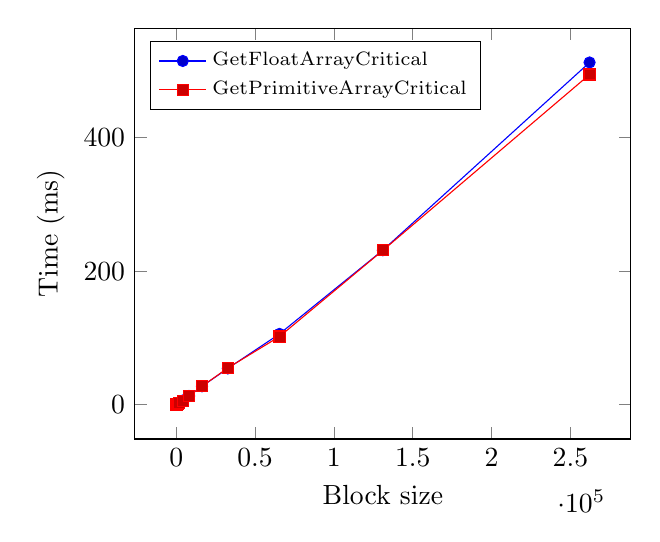
\begin{tikzpicture}
\begin{axis}[xlabel={Block size},ylabel={Time (ms)},width=0.65\linewidth,legend pos=north west,scaled y ticks = false,legend cell align=left,legend style={font=\scriptsize}]
\addplot coordinates {
(16, 0.0187)
(32, 0.0347)
(64, 0.0709)
(128, 0.1447)
(256, 0.3014)
(512, 0.6505)
(1024, 1.3689)
(2048, 2.9279)
(4096, 6.2499)
(8192, 13.1419)
(16384, 27.7314)
(32768, 54.4151)
(65536, 106.1420)
(131072, 231.5323)
(262144, 512.7674)
};
\addplot coordinates {
(16, 0.0202)
(32, 0.0368)
(64, 0.0705)
(128, 0.1434)
(256, 0.2978)
(512, 0.6379)
(1024, 1.3437)
(2048, 2.8773)
(4096, 6.1206)
(8192, 13.2345)
(16384, 27.6080)
(32768, 55.1227)
(65536, 102.1585)
(131072, 231.2663)
(262144, 494.7038)
};
\legend{GetFloatArrayCritical, GetPrimitiveArrayCritical}
\end{axis}
\end{tikzpicture}

% \end{table}
%
% \begin{table}[H]
%     \centering
%     \label{tab:cpp:columbia:iterative}
%     \caption{C++ Columbia Iterative, Time (ms)}
%     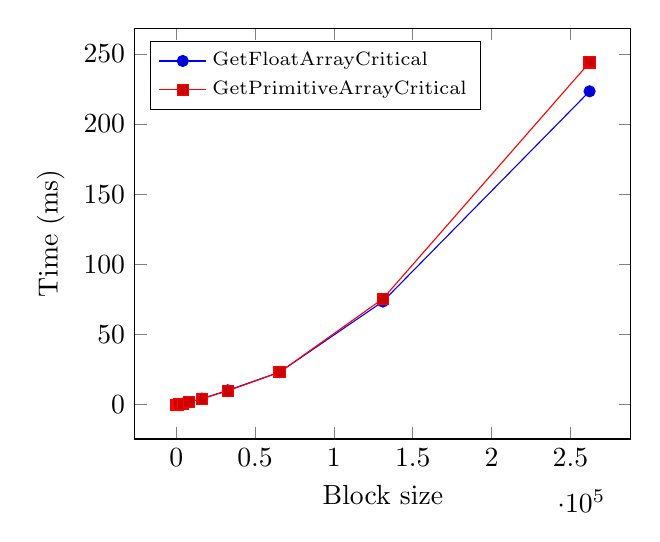
\begin{tikzpicture}
\begin{axis}[xlabel={Block size},ylabel={Time (ms)},width=0.65\linewidth,legend pos=north west,scaled y ticks = false,legend cell align=left,legend style={font=\scriptsize}]
\addplot coordinates {
(16, 0.0057)
(32, 0.0070)
(64, 0.0092)
(128, 0.0136)
(256, 0.0222)
(512, 0.0418)
(1024, 0.0970)
(2048, 0.2761)
(4096, 0.7818)
(8192, 1.8794)
(16384, 4.3304)
(32768, 10.2608)
(65536, 23.1917)
(131072, 73.5225)
(262144, 223.3088)
};
\addplot coordinates {
(16, 0.0072)
(32, 0.0086)
(64, 0.0083)
(128, 0.0115)
(256, 0.0200)
(512, 0.0366)
(1024, 0.0773)
(2048, 0.2604)
(4096, 0.7974)
(8192, 1.9326)
(16384, 4.2789)
(32768, 9.9388)
(65536, 23.1031)
(131072, 75.4942)
(262144, 243.8496)
};
\legend{GetFloatArrayCritical, GetPrimitiveArrayCritical}
\end{axis}
\end{tikzpicture}

% \end{table}
%
% \begin{table}[H]
%     \centering
%     \label{tab:cpp:kiss}
%     \caption{C++ KISS, Time (ms)}
%     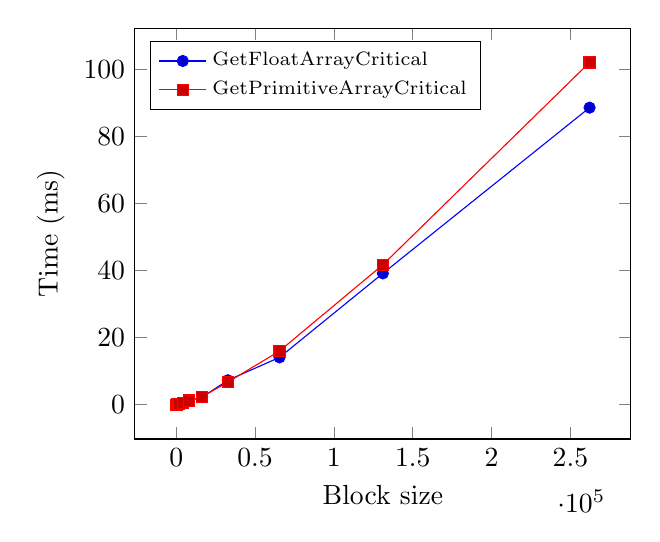
\begin{tikzpicture}
\begin{axis}[xlabel={Block size},ylabel={Time (ms)},width=0.65\linewidth,legend pos=north west,scaled y ticks = false,legend cell align=left,legend style={font=\scriptsize}]
\addplot coordinates {
(16, 0.0050)
(32, 0.0060)
(64, 0.0072)
(128, 0.0139)
(256, 0.0212)
(512, 0.0478)
(1024, 0.0885)
(2048, 0.1965)
(4096, 0.3867)
(8192, 1.1701)
(16384, 2.2685)
(32768, 7.2940)
(65536, 14.1297)
(131072, 39.1887)
(262144, 88.6356)
};
\addplot coordinates {
(16, 0.0056)
(32, 0.0069)
(64, 0.0079)
(128, 0.0131)
(256, 0.0182)
(512, 0.0461)
(1024, 0.0992)
(2048, 0.2047)
(4096, 0.4022)
(8192, 1.2470)
(16384, 2.3713)
(32768, 6.7420)
(65536, 16.0281)
(131072, 41.7620)
(262144, 102.1196)
};
\legend{GetFloatArrayCritical, GetPrimitiveArrayCritical}
\end{axis}
\end{tikzpicture}

% \end{table}
% \begin{table}
%     \centering
%     \label{tab:cpp:columbia:iterative:optimized}
%     \caption{C++ Columbia Iterative Optimized, Time (ms)}
%     \input{Data/results/FFT/CPP_Columbia_optimized.tex}
% \end{table}

% \begin{table}
%     \centering
%     \label{fig:java:columbia:iterative:optimized}
%     \caption{Label here}
%     \input{Data/results/FFT/Java_Columbia_optimized_Iterative.tex}
% \end{table}

% \section{Bar charts}

% \begin{figure}
%     \centering
%     \input{Data/results/FFT/Java_Princeton_Recursive_barchart.tex}
%     \label{fig:java:princeton:recursive:barchart}
%     \caption{Java Princeton Recursive bar chart}
% \end{figure}

\section{ARR}

\begin{table}[H]
    \centering
    \caption{Common table for ARR C++ tests, Time(ms)}
    \label{tab:appendix:common:arr}
    \rotatebox{90}{
        \resizebox{\columnwidth}{!}{
            \rowcolors{1}{}{lightgray}
\begin{tabular}{lrrrrrrrrr}\toprule
\textbf{Block size}  & \textbf{Columbia Iterative} & \textbf{Float Columbia Iterative} & \textbf{Float Princeton Iterative} & \textbf{Float Princeton Recursive} & \textbf{KISS} & \textbf{NEON Iterative} & \textbf{NEON Recursive} & \textbf{Princeton Iterative} & \textbf{Princeton Recursive}\\\midrule
\textbf{16}  & 0.0057 $\pm$ 0.0004 & 0.0039 $\pm$ 0.0002 & 0.0073 $\pm$ 0.0004 & 0.0220 $\pm$ 0.0090 & 0.0050 $\pm$ 0.0010 & 0.0045 $\pm$ 0.0010 & 0.0079 $\pm$ 0.0006 & 0.0083 $\pm$ 0.0008 & 0.0187 $\pm$ 0.0006\\
\textbf{32}  & 0.0070 $\pm$ 0.0002 & 0.0046 $\pm$ 0.0008 & 0.0110 $\pm$ 0.0008 & 0.0318 $\pm$ 0.0006 & 0.0060 $\pm$ 0.0002 & 0.0048 $\pm$ 0.0008 & 0.0106 $\pm$ 0.0004 & 0.0124 $\pm$ 0.0010 & 0.0347 $\pm$ 0.0002\\
\textbf{64}  & 0.0092 $\pm$ 0.0002 & 0.0053 $\pm$ 0.0001 & 0.0169 $\pm$ 0.0002 & 0.0617 $\pm$ 0.0002 & 0.0072 $\pm$ 0.0002 & 0.0055 $\pm$ 0.0002 & 0.0162 $\pm$ 0.0004 & 0.0201 $\pm$ 0.0006 & 0.0709 $\pm$ 0.0022\\
\textbf{128}  & 0.0136 $\pm$ 0.0010 & 0.0077 $\pm$ 0.0002 & 0.0310 $\pm$ 0.0010 & 0.1267 $\pm$ 0.0008 & 0.0139 $\pm$ 0.0004 & 0.0087 $\pm$ 0.0010 & 0.0280 $\pm$ 0.0012 & 0.0348 $\pm$ 0.0004 & 0.1447 $\pm$ 0.0016\\
\textbf{256}  & 0.0222 $\pm$ 0.0022 & 0.0126 $\pm$ 0.0002 & 0.0572 $\pm$ 0.0010 & 0.2637 $\pm$ 0.0024 & 0.0212 $\pm$ 0.0020 & 0.0137 $\pm$ 0.0004 & 0.0506 $\pm$ 0.0020 & 0.0651 $\pm$ 0.0010 & 0.3014 $\pm$ 0.0024\\
\textbf{512}  & 0.0418 $\pm$ 0.0010 & 0.0243 $\pm$ 0.0016 & 0.1138 $\pm$ 0.0114 & 0.5549 $\pm$ 0.0108 & 0.0478 $\pm$ 0.0024 & 0.0312 $\pm$ 0.0004 & 0.1036 $\pm$ 0.0088 & 0.1275 $\pm$ 0.0022 & 0.6505 $\pm$ 0.0037\\
\textbf{1024}  & 0.0970 $\pm$ 0.0100 & 0.0512 $\pm$ 0.0012 & 0.2180 $\pm$ 0.0024 & 1.1660 $\pm$ 0.0057 & 0.0885 $\pm$ 0.0120 & 0.0667 $\pm$ 0.0106 & 0.1917 $\pm$ 0.0025 & 0.2659 $\pm$ 0.0027 & 1.3689 $\pm$ 0.0122\\
\textbf{2048}  & 0.2761 $\pm$ 0.0102 & 0.1330 $\pm$ 0.0427 & 0.4184 $\pm$ 0.0031 & 2.4295 $\pm$ 0.0065 & 0.1965 $\pm$ 0.0045 & 0.1327 $\pm$ 0.0061 & 0.3825 $\pm$ 0.0229 & 0.5235 $\pm$ 0.0045 & 2.9279 $\pm$ 0.0419\\
\textbf{4096}  & 0.7818 $\pm$ 0.0161 & 0.3549 $\pm$ 0.0180 & 0.8859 $\pm$ 0.0061 & 5.1699 $\pm$ 0.0310 & 0.3867 $\pm$ 0.0080 & 0.3437 $\pm$ 0.0120 & 0.7539 $\pm$ 0.0076 & 1.1475 $\pm$ 0.0118 & 6.2499 $\pm$ 0.0496\\
\textbf{8192}  & 1.8794 $\pm$ 0.0417 & 2.0429 $\pm$ 0.1697 & 2.0668 $\pm$ 0.0122 & 10.8915 $\pm$ 0.0457 & 1.1701 $\pm$ 0.0504 & 1.0274 $\pm$ 0.0241 & 1.6084 $\pm$ 0.0212 & 2.6441 $\pm$ 0.0904 & 13.1419 $\pm$ 0.1317\\
\textbf{16384}  & 4.3304 $\pm$ 0.1374 & 5.1738 $\pm$ 0.6893 & 4.4843 $\pm$ 0.0292 & 22.8474 $\pm$ 0.1262 & 2.2685 $\pm$ 0.0764 & 2.0687 $\pm$ 0.0239 & 3.3681 $\pm$ 0.0674 & 5.5785 $\pm$ 0.2309 & 27.7314 $\pm$ 0.1439\\
\textbf{32768}  & 10.2608 $\pm$ 0.3557 & 7.4332 $\pm$ 0.2993 & 9.6815 $\pm$ 0.1135 & 33.4821 $\pm$ 0.6149 & 7.2940 $\pm$ 0.2756 & 4.3371 $\pm$ 0.0702 & 7.3011 $\pm$ 0.1803 & 12.1775 $\pm$ 0.4559 & 54.4151 $\pm$ 1.4030\\
\textbf{65536}  & 23.1917 $\pm$ 0.6235 & 22.0037 $\pm$ 3.0306 & 20.5733 $\pm$ 0.4116 & 93.5059 $\pm$ 2.8971 & 14.1297 $\pm$ 0.2103 & 11.5128 $\pm$ 0.2544 & 15.6232 $\pm$ 0.3387 & 27.1549 $\pm$ 0.8795 & 106.1420 $\pm$ 3.5200\\
\textbf{131072}  & 73.5225 $\pm$ 1.2326 & 46.3222 $\pm$ 6.9762 & 45.3676 $\pm$ 0.9706 & 192.1138 $\pm$ 8.2559 & 39.1887 $\pm$ 0.4663 & 28.9012 $\pm$ 0.6358 & 33.8117 $\pm$ 0.4263 & 76.6735 $\pm$ 1.4996 & 231.5323 $\pm$ 6.8488\\
\textbf{262144} & 223.3088 $\pm$ 0.6968 & 136.4392 $\pm$ 2.0163 & 128.3593 $\pm$ 1.9263 & 372.1897 $\pm$ 16.2894 & 88.6356 $\pm$ 0.7389 & 67.5020 $\pm$ 1.6435 & 70.9477 $\pm$ 0.6299 & 210.3414 $\pm$ 1.4461 & 512.7674 $\pm$ 11.1828\\
\bottomrule
\end{tabular}

        }
    }
\end{table}

\begin{table}[H]
    \centering
    \begin{tabular}{cc}
        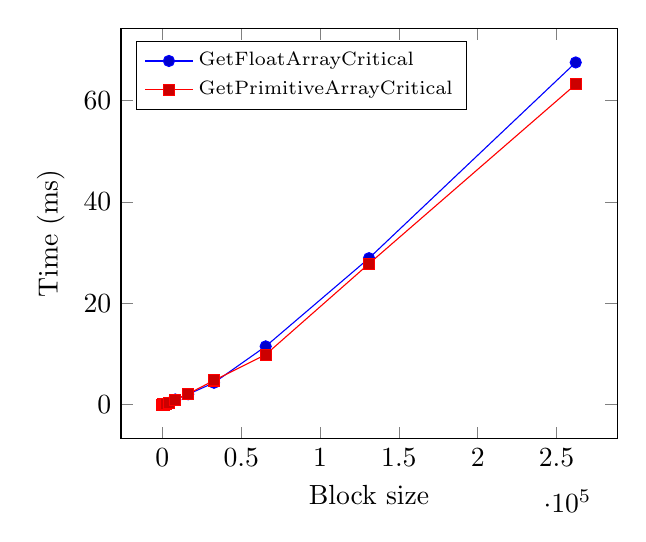
\begin{tikzpicture}
\begin{axis}[xlabel={Block size},ylabel={Time (ms)},width=0.65\linewidth,legend pos=north west,scaled y ticks = false,legend cell align=left,legend style={font=\scriptsize}]
\addplot coordinates {
(16, 0.0045)
(32, 0.0048)
(64, 0.0055)
(128, 0.0087)
(256, 0.0137)
(512, 0.0312)
(1024, 0.0667)
(2048, 0.1327)
(4096, 0.3437)
(8192, 1.0274)
(16384, 2.0687)
(32768, 4.3371)
(65536, 11.5128)
(131072, 28.9012)
(262144, 67.5020)
};
\addplot coordinates {
(16, 0.0057)
(32, 0.0050)
(64, 0.0056)
(128, 0.0089)
(256, 0.0134)
(512, 0.0348)
(1024, 0.0608)
(2048, 0.1925)
(4096, 0.3656)
(8192, 1.0051)
(16384, 2.1559)
(32768, 4.7898)
(65536, 9.8807)
(131072, 27.8158)
(262144, 63.1858)
};
\legend{GetFloatArrayCritical, GetPrimitiveArrayCritical}
\end{axis}
\end{tikzpicture}

        &
        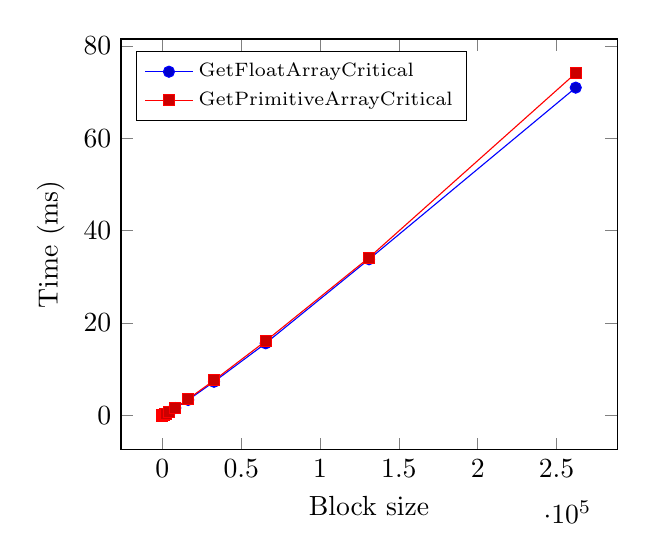
\begin{tikzpicture}
\begin{axis}[xlabel={Block size},ylabel={Time (ms)},width=0.65\linewidth,legend pos=north west,scaled y ticks = false,legend cell align=left,legend style={font=\scriptsize}]
\addplot coordinates {
(16, 0.0079)
(32, 0.0106)
(64, 0.0162)
(128, 0.0280)
(256, 0.0506)
(512, 0.1036)
(1024, 0.1917)
(2048, 0.3825)
(4096, 0.7539)
(8192, 1.6084)
(16384, 3.3681)
(32768, 7.3011)
(65536, 15.6232)
(131072, 33.8117)
(262144, 70.9477)
};
\addplot coordinates {
(16, 0.0108)
(32, 0.0150)
(64, 0.0187)
(128, 0.0286)
(256, 0.0544)
(512, 0.0961)
(1024, 0.1868)
(2048, 0.3659)
(4096, 0.8086)
(8192, 1.6133)
(16384, 3.5690)
(32768, 7.6009)
(65536, 16.1129)
(131072, 34.1650)
(262144, 74.0746)
};
\legend{GetFloatArrayCritical, GetPrimitiveArrayCritical}
\end{axis}
\end{tikzpicture}

        \\
        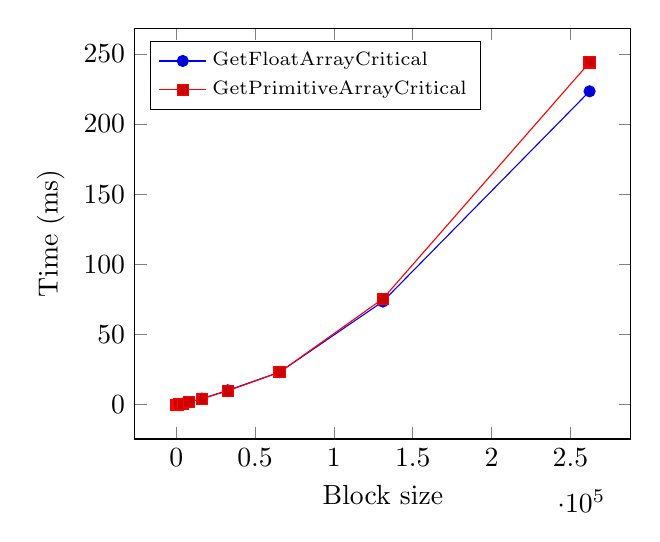
\begin{tikzpicture}
\begin{axis}[xlabel={Block size},ylabel={Time (ms)},width=0.65\linewidth,legend pos=north west,scaled y ticks = false,legend cell align=left,legend style={font=\scriptsize}]
\addplot coordinates {
(16, 0.0057)
(32, 0.0070)
(64, 0.0092)
(128, 0.0136)
(256, 0.0222)
(512, 0.0418)
(1024, 0.0970)
(2048, 0.2761)
(4096, 0.7818)
(8192, 1.8794)
(16384, 4.3304)
(32768, 10.2608)
(65536, 23.1917)
(131072, 73.5225)
(262144, 223.3088)
};
\addplot coordinates {
(16, 0.0072)
(32, 0.0086)
(64, 0.0083)
(128, 0.0115)
(256, 0.0200)
(512, 0.0366)
(1024, 0.0773)
(2048, 0.2604)
(4096, 0.7974)
(8192, 1.9326)
(16384, 4.2789)
(32768, 9.9388)
(65536, 23.1031)
(131072, 75.4942)
(262144, 243.8496)
};
\legend{GetFloatArrayCritical, GetPrimitiveArrayCritical}
\end{axis}
\end{tikzpicture}

        &
        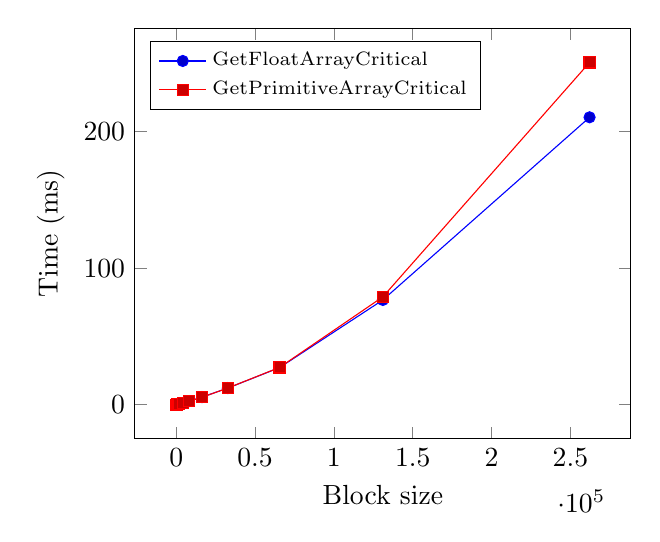
\begin{tikzpicture}
\begin{axis}[xlabel={Block size},ylabel={Time (ms)},width=0.65\linewidth,legend pos=north west,scaled y ticks = false,legend cell align=left,legend style={font=\scriptsize}]
\addplot coordinates {
(16, 0.0083)
(32, 0.0124)
(64, 0.0201)
(128, 0.0348)
(256, 0.0651)
(512, 0.1275)
(1024, 0.2659)
(2048, 0.5235)
(4096, 1.1475)
(8192, 2.6441)
(16384, 5.5785)
(32768, 12.1775)
(65536, 27.1549)
(131072, 76.6735)
(262144, 210.3414)
};
\addplot coordinates {
(16, 0.0097)
(32, 0.0132)
(64, 0.0214)
(128, 0.0342)
(256, 0.0627)
(512, 0.1225)
(1024, 0.2744)
(2048, 0.5257)
(4096, 1.1701)
(8192, 2.5845)
(16384, 5.4518)
(32768, 12.2266)
(65536, 27.2805)
(131072, 78.9501)
(262144, 250.4870)
};
\legend{GetFloatArrayCritical, GetPrimitiveArrayCritical}
\end{axis}
\end{tikzpicture}

        \\
        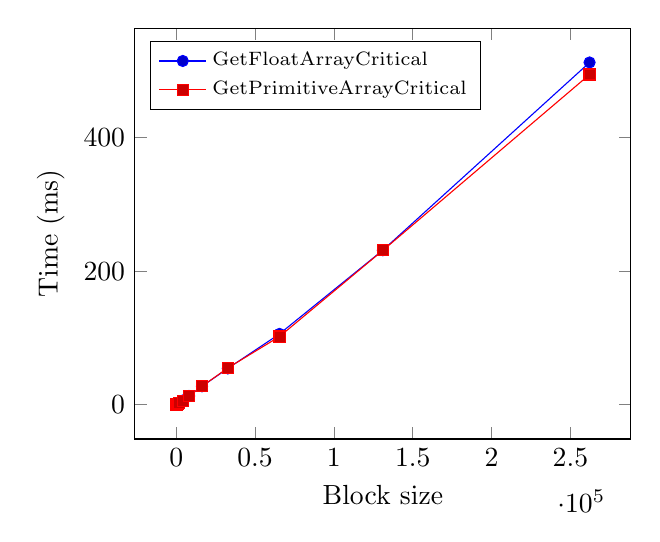
\begin{tikzpicture}
\begin{axis}[xlabel={Block size},ylabel={Time (ms)},width=0.65\linewidth,legend pos=north west,scaled y ticks = false,legend cell align=left,legend style={font=\scriptsize}]
\addplot coordinates {
(16, 0.0187)
(32, 0.0347)
(64, 0.0709)
(128, 0.1447)
(256, 0.3014)
(512, 0.6505)
(1024, 1.3689)
(2048, 2.9279)
(4096, 6.2499)
(8192, 13.1419)
(16384, 27.7314)
(32768, 54.4151)
(65536, 106.1420)
(131072, 231.5323)
(262144, 512.7674)
};
\addplot coordinates {
(16, 0.0202)
(32, 0.0368)
(64, 0.0705)
(128, 0.1434)
(256, 0.2978)
(512, 0.6379)
(1024, 1.3437)
(2048, 2.8773)
(4096, 6.1206)
(8192, 13.2345)
(16384, 27.6080)
(32768, 55.1227)
(65536, 102.1585)
(131072, 231.2663)
(262144, 494.7038)
};
\legend{GetFloatArrayCritical, GetPrimitiveArrayCritical}
\end{axis}
\end{tikzpicture}

        &
        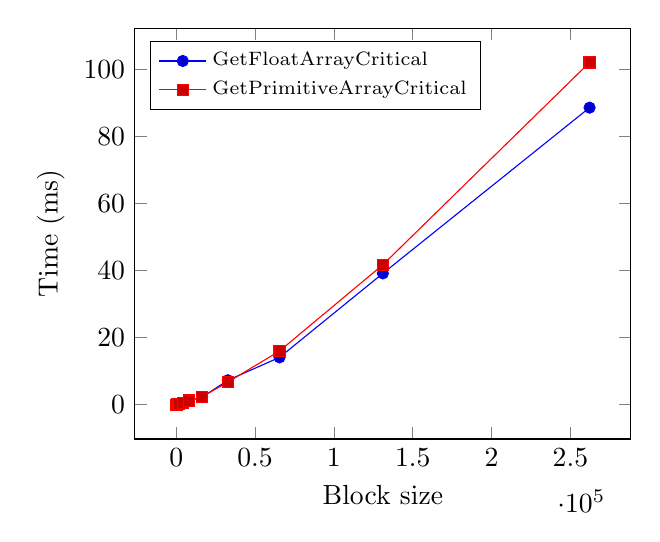
\begin{tikzpicture}
\begin{axis}[xlabel={Block size},ylabel={Time (ms)},width=0.65\linewidth,legend pos=north west,scaled y ticks = false,legend cell align=left,legend style={font=\scriptsize}]
\addplot coordinates {
(16, 0.0050)
(32, 0.0060)
(64, 0.0072)
(128, 0.0139)
(256, 0.0212)
(512, 0.0478)
(1024, 0.0885)
(2048, 0.1965)
(4096, 0.3867)
(8192, 1.1701)
(16384, 2.2685)
(32768, 7.2940)
(65536, 14.1297)
(131072, 39.1887)
(262144, 88.6356)
};
\addplot coordinates {
(16, 0.0056)
(32, 0.0069)
(64, 0.0079)
(128, 0.0131)
(256, 0.0182)
(512, 0.0461)
(1024, 0.0992)
(2048, 0.2047)
(4096, 0.4022)
(8192, 1.2470)
(16384, 2.3713)
(32768, 6.7420)
(65536, 16.0281)
(131072, 41.7620)
(262144, 102.1196)
};
\legend{GetFloatArrayCritical, GetPrimitiveArrayCritical}
\end{axis}
\end{tikzpicture}

    \end{tabular}
    \caption{ARR C++}
    \label{fig:appendix:arr:line}
\end{table}
